\chapter{Concept Development}
\label{chap:concept-development}

\section{Revisiting the problem definition}



\section{Understanding crowd safety management}
\label{sec:crowd-safety}

In order to develop a solution that supports crowd safety professionals, it is imperative to understand how they operate, and what tools they currently have at their disposal. Together with my co-founders at Fluxense, we conducted interviews with many crowd safety professionals from various different organizations, including Event Safety (Smukfest), smash! bang! pow! (Syd for Solen), Roskilde Festival, and Live Nation (Copenhell, Heartland) -- see appendix \ref{appendix:rf-meeting-notes} for meeting notes. Throughout this period, it became clearer that crowd safety management is very complex, and is almost as much a philosophy as it is a science. Music festivals and events vary greatly in size, participant demographics, venues, and budget. Equally varied are the crowd safety professionals themselves, who appeared to have varying levels of experience, as well as distinct approaches to their work.

Most interestingly, the greatest discrepancy was seemingly between a focus on incident-prevention and incident-response, or "crowd safety vs. security", as according to Roskilde Festival's Director of Safety, Morten Therkildsen. A security-focused approach often involves less planning, as well as hiring third-party professionals to handle safety during the event. Safety-focused teams, on the other hand, spend most of the year leading up to their events meticulously planning initiatives to ensure the well-being and enjoyment of their guests. The distinction between these two protocols was apparent throughout Fluxense's collaborations with both Copenhell and Roskilde Festival. At their 2024 events, Live Nation had two full-time employees responsible for crowd safety at Copenhell, whereas Roskilde Festival had a team of 10+ full-time employees.

\subsection{Existing frameworks and workflows}

\subsection{Key metrics}



\section{Comparing technical solutions}

\subsection{Global Positioning System (GPS)}
\label{sec:gps}

Using GPS to track the location of festival-goers is a common practice, and likely the easiest to implement technology in this comparison. This is typically achieved by providing guests with a mobile app that uses their smartphone's GPS to track their location. Of course, this requires the guests to opt in to location tracking, as well as there being a sufficient reason for doing so. In almost all cases, this is attempted by including a map of the festival in the app, as visible in Figure \ref{fig:festival_apps}. This feature, however, still functions without location tracking, and therefore doesn't guarantee users will grant data access. Even before this obstacle is met, there is the question of whether festival-goers will actually use the app. A study on Roskilde Festival 2015 by the Copenhagen Business School  found that of the 60 thousand people who installed the festival application, 44 thousand opted-in to allowing anonymous tracking; yielding 38.678 unique users who were present inside the festival area \cite{rf_app}. This equates to slightly under 30\% of the total 130 thousand attendees. In a crowd safety context, this is a significant limitation, as the location data gathered is not representative of entire crowds.

\begin{figure}[H]
  \centering
  \begin{subfigure}{.3\textwidth}
    \centering
    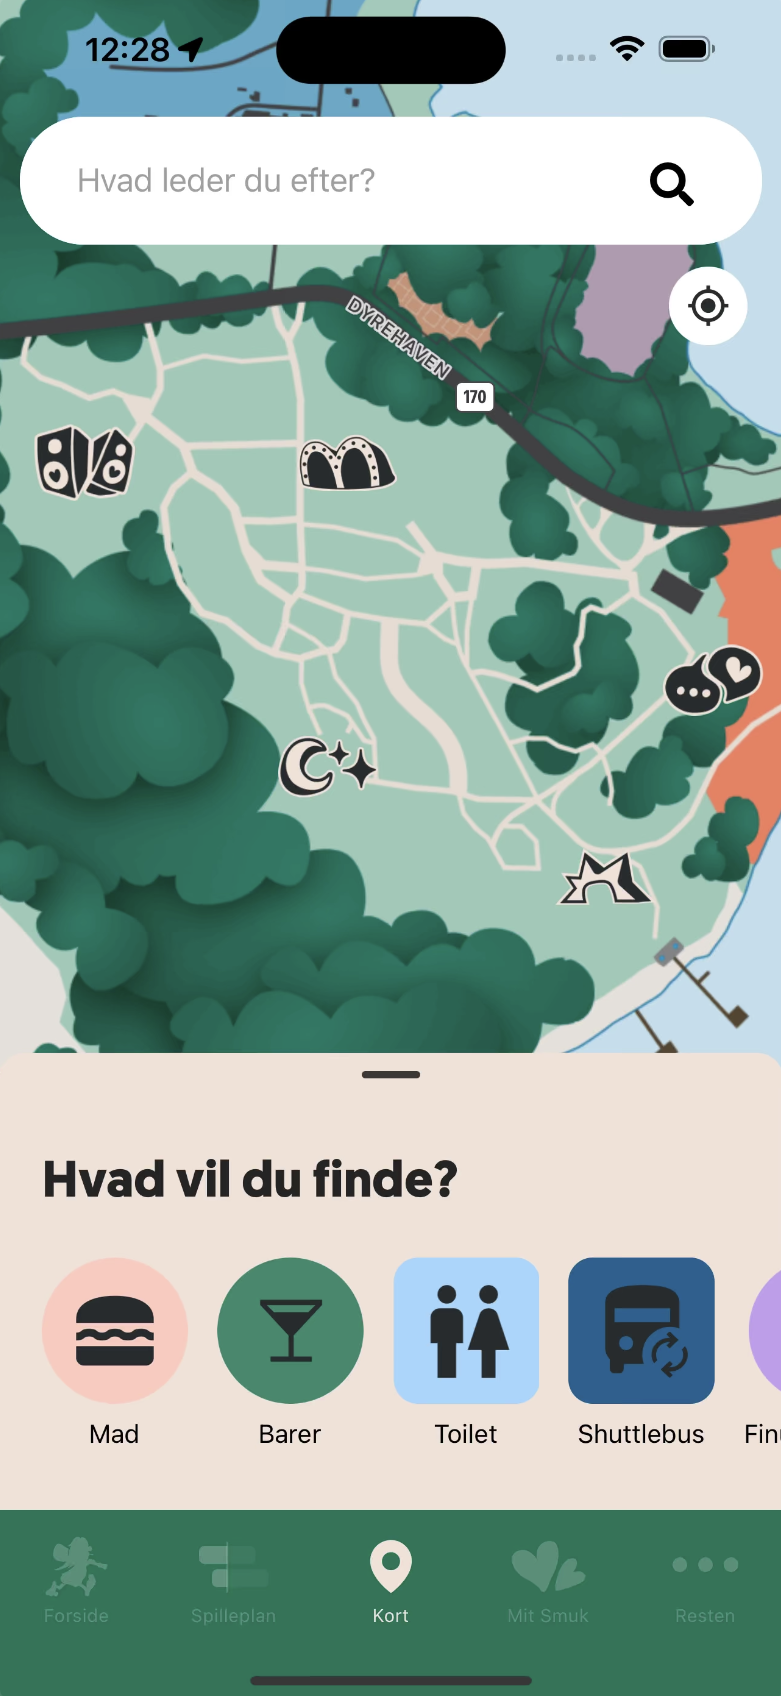
\includegraphics[width=4cm]{Pictures/Misc/smukfest_app.png}
    \caption{Smukfest app \cite{smukfest_app}}
    \label{fig:smukfest_app}
  \end{subfigure}%
  \begin{subfigure}{.3\textwidth}
    \centering
    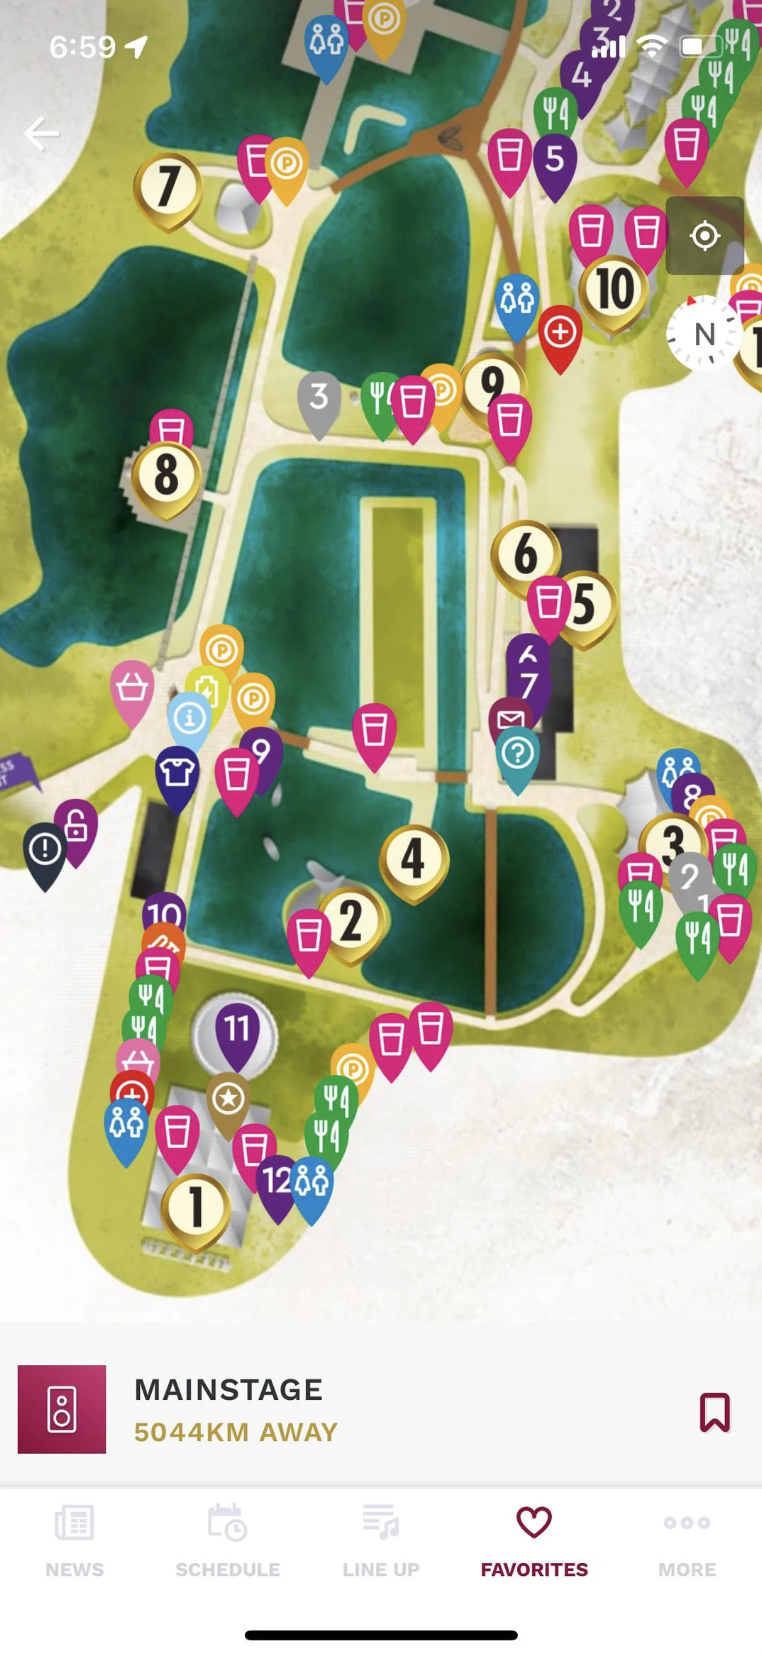
\includegraphics[width=4cm]{Pictures/Misc/tomorrowland_app.png}
    \caption{Tomorrowland app \cite{tomorrowland_app}}
    \label{fig:tomorrowland_app}
  \end{subfigure}
  \begin{subfigure}{.3\textwidth}
    \centering
    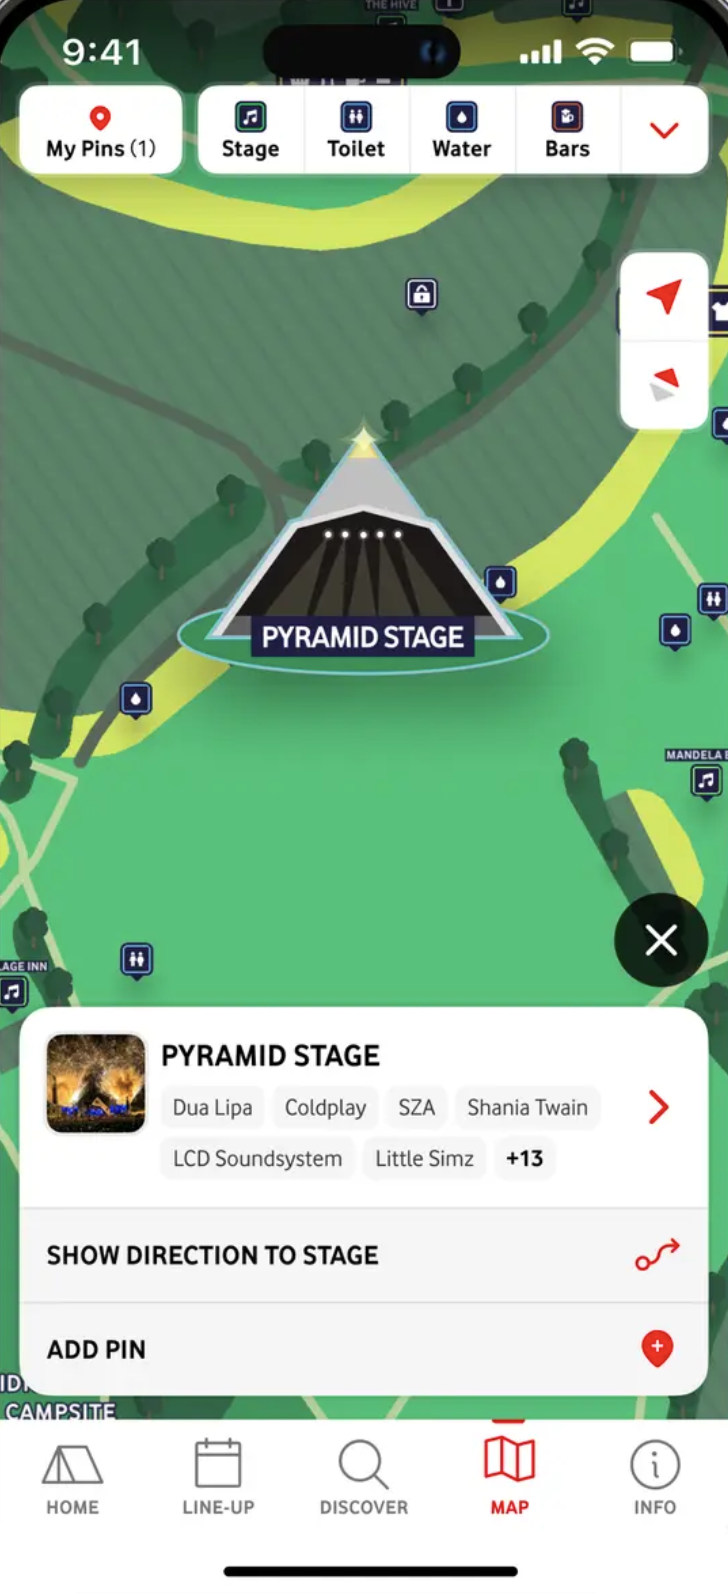
\includegraphics[width=4cm]{Pictures/Misc/glastonbury_app.png}
    \caption{Glastonbury app \cite{glastonbury_app}}
    \label{fig:glastonbury_app}
  \end{subfigure}
  \caption{Examples of map features in music festival mobile apps (Smukfest, Tomorrowland, Glastonbury), often used to encourage attendees to enable GPS location tracking.}
  \label{fig:festival_apps}
\end{figure}


Beyond low adoption and potential privacy concerns, the technical limitations of GPS also hinder its utility for detailed crowd analysis. According to GPS.gov, GPS-enabled smartphones are typically accurate only to within a 4.9 m radius under open sky; however, their accuracy worsens near buildings, bridges, and trees \cite{gps}. While a 4.9-meter radius might seem acceptable for general location awareness on a festival map, this level of uncertainty significantly hinders the calculation of precise crowd dynamics metrics. Furthermore, the degradation of accuracy near structures is particularly problematic in festival environments, which often feature large stages, tents, and temporary structures -- precisely where accurate monitoring is most needed. The effectiveness of GPS tracking is also contingent on factors outside the organizers' control, such as users keeping their phones charged and maintaining a stable mobile data connection.

Compared to infrastructure-based monitoring systems (like cameras or dedicated sensors), GPS relies heavily on user cooperation and device functionality, making it less suitable for generating the consistent, high-resolution data needed for proactive crowd safety management and detailed post-event analysis. Therefore, while mobile app GPS data can offer some high-level insights into general attendee distribution, its inherent limitations in accuracy make it insufficient as a primary tool for gathering crowd dynamics measurements.

\subsection{Bluetooth beacons}
Another potential solution for gathering crowd dynamics data involves utilizing Bluetooth Low Energy (BLE), a wireless communication technology designed for low power consumption. This technology is typically utilized in Bluetooth beacons -- devices that periodically transmit signals that can be detected by nearby receivers, such as smartphones or dedicated hardware. These signals can be used to determine the proximity of beacons to the receivers, as well as location estimation through triangulation techniques, requiring three or more receivers. This capability is increasingly utilized for proximity marketing, indoor navigation, and positional tracking, typically in retail environments \cite{bt_beacon}. It has also been effectively used for guest tracking in environments like museums, as demonstrated in a study at the Galleria Borghese, where visitors were given portable BLE beacons tracked by fixed receivers \cite{borghese}.

Finding examples of BLE beacons utilized at large outdoor events is more challenging, as the technology has its own set of drawbacks. Similar to GPS-based mobile apps, the effectiveness of Bluetooth beacon systems is significantly contingent on user cooperation. Beacons can be implemented either as dedicated physical devices or embedded within smartphone applications. The latter is simpler and cheaper, however motiving users to install an app is challenging, as discussed in section \ref{sec:gps}. The former approach has challenges of its own, as requiring event participants to carry a dedicated device demands a value proposition of its own, not to mention the overhead costs involved in developing, deploying, and maintaining the system. Given that beacon signals have an effective range of 30 meters without obstructions, a considerable number of receivers are necessary to ensure adequate coverage \cite{bt_beacon}.

Ultimately, the most critical factor for crowd dynamics analysis is the technology's accuracy. A study conducted at a large exhibition in Japan evaluated the accuracy of trajectory estimation using Bluetooth beacons. They found that  in 68\% of instances, their positional estimates were accurate within a radius of 18 meters \cite{bt_japan}. While still useful for certain applications like indoor tracking or general zone classification, this level of accuracy is significantly less precise than typically achievable with GPS (section \ref{sec:gps}). This limitation, combined with the dependency on user adoption and implementation costs, makes Bluetooth beacons a less favorable option for gathering crowd dynamics data at large outdoor events.

\subsection{Camera solutions}
Camera-based solutions leverage existing CCTV systems in conjunction with computer vision algorithms to analyze crowd dynamics. Utilizing video footage from these camera systems, novel advancements in machine learning and computer vision enable automated extraction of valuable metrics.

A primary advantage of this approach compared to GPS (Section 2.3.1) and Bluetooth beacon (Section 2.3.2) systems is its independence from attendee cooperation. Unlike solutions requiring festival-goers to install an app, enable location services, carry a specific device, or keep their phones charged, camera-based analysis operates passively. It gathers data from anyone within the camera's field of view, potentially offering a more comprehensive and unbiased view of crowd behavior across monitored areas. This circumvents the significant limitations associated with low adoption rates and opt-in requirements inherent in user-device-dependent methods.

(competitor analysis)

\section{Proposed solution}
\label{sec:solution}

% also state which areas will be monitored and analyzed

\section{Feasibility of solution}
\label{sec:feasibility}
\subsection{Technical feasibility}
\subsection{Legal feasibility}
When dealing with CCTV footage, there are a number of legal considerations to take into account.

\subsection{Financial feasibility}


